% !TeX spellcheck = en_GB
% !TeX program = lualatex
%
% v 2.3  Feb 2019   Volker RW Schaa
%		# changes in the collaboration therefore updated file "jacow-collaboration.tex"
%		# all References with DOIs have their period/full stop before the DOI (after pp. or year)
%		# in the author/affiliation block all ZIP codes in square brackets removed as it was not %         understood as optional parameter and ZIP codes had bin put in brackets
%       # References to the current IPAC are changed to "IPAC'19, Melbourne, Australia"
%       # font for ‘url’ style changed to ‘newtxtt’ as it is easier to distinguish "O" and "0"
%
\documentclass[a4paper,
               %boxit,        % check whether paper is inside correct margins
               %titlepage,    % separate title page
               %refpage       % separate references
               %biblatex,     % biblatex is used
               keeplastbox,   % flushend option: not to un-indent last line in References
               %nospread,     % flushend option: do not fill with whitespace to balance columns
               %hyphens,      % allow \url to hyphenate at "-" (hyphens)
               %xetex,        % use XeLaTeX to process the file
               %luatex,       % use LuaLaTeX to process the file
               ]{jacow}
%
% ONLY FOR \footnote in table/tabular
%
\usepackage{pdfpages,multirow,ragged2e} %
\usepackage{tablefootnote}
%
% CHANGE SEQUENCE OF GRAPHICS EXTENSION TO BE EMBEDDED
% ----------------------------------------------------
% test for XeTeX where the sequence is by default eps-> pdf, jpg, png, pdf, ...
%    and the JACoW template provides JACpic2v3.eps and JACpic2v3.jpg which
%    might generates errors, therefore PNG and JPG first
%
\makeatletter%
	\ifboolexpr{bool{xetex}}
	 {\renewcommand{\Gin@extensions}{.pdf,%
	                    .png,.jpg,.bmp,.pict,.tif,.psd,.mac,.sga,.tga,.gif,%
	                    .eps,.ps,%
	                    }}{}
\makeatother
\newcommand{\ts}{\textsuperscript}
% CHECK FOR XeTeX/LuaTeX BEFORE DEFINING AN INPUT ENCODING
% --------------------------------------------------------
%   utf8  is default for XeTeX/LuaTeX
%   utf8  in LaTeX only realises a small portion of codes
%
\ifboolexpr{bool{xetex} or bool{luatex}} % test for XeTeX/LuaTeX
 {}                                      % input encoding is utf8 by default
 {\usepackage[utf8]{inputenc}}           % switch to utf8

\usepackage[USenglish]{babel}
\usepackage{subcaption}

%
% if BibLaTeX is used
%
\ifboolexpr{bool{jacowbiblatex}}%
 {%
  \addbibresource{jacow-test.bib}
  \addbibresource{biblatex-examples.bib}
 }{}
\listfiles

%%
%%   Lengths for the spaces in the title
%%   \setlength\titleblockstartskip{..}  %before title, default 3pt
%%   \setlength\titleblockmiddleskip{..} %between title + author, default 1em
%%   \setlength\titleblockendskip{..}    %afterauthor, default 1em

\begin{document}

\title{Medida da tabela de feedforward do Wiggler W180}

\author{Envolvidos: Ximenes Resende, Gabriel da Ascenção, Rafael Lyra, Murilo Alves \\ FAC - LNLS \\ Terça-feira, 20 de setembro de 2022}
\maketitle
%
\section{Resumo}
Continuação dos estudos de caracterizações do efeito do wiggler W180 no feixe do anel de armazenamento. Neste estudo foi medida a tabela de feedforward das corretoras do wiggler para minimizar as distorções de órbita causadas pelas primeiras e segundas integrais deste ID. 

\section{Procedimento de medida}

\begin{enumerate}
    \item Zerar correntes das corretoras de feedforward
    \item Mover o gap do wiggler para o máximo ($\SI{300}{\milli\meter}$)
    \item Corrigir a órbita com o SOFB e registrar os kicks iniciais $\left(\vec{\theta}_{x, 0}, \vec{\theta}_{y, 0}\right)$
    \item Mover o gap do ondulador para o valor de interesse, com isso a órbita será distorcida
    \item Corrigir a órbita com o SOFB. Esta etapa é necessária para medir a matriz resposta próximo da órbita ideal
    \item Medir a matriz resposta de órbita das duas corretoras do wiggler
    \item Desfazer a correção feita com o SOFB, reaplicando os kicks iniciais que foram registrados $\left(\vec{\theta}_{x, 0}, \vec{\theta}_{y, 0}\right)$
    \item Com a matriz resposta das corretoras feedforward, calcular e aplicar iterativamente os kicks necessários para corrigir a distorção gerada pelo wiggler na fase de interesse. 
    \item Após convergência da correção de órbita com as corretoras feedforward, registrar kicks $\left(\theta_{x, \mathrm{CH1}},\theta_{x, \mathrm{CH2}}\right)$ para o gap avaliado
\end{enumerate}

Seguindo o procedimento descrito, cria-se uma tabela de kicks $\left(\theta_{x, \mathrm{CH1}},\theta_{x, \mathrm{CH2}}\right)$ em função do gap do wiggler.

As etapas 2 e 3 podem ser realizadas apenas no processo para medir o primeiro valor de gap. Uma vez registrados os kicks iniciais uma vez, eles podem ser utilizados como referência para medidas em outros gaps. 

Outra observação importante é que com este procedimento, estamos convencionando que para o gap máximo do wiggler de $\SI{300}{\milli\meter}$, as correntes das corretoras serão zero.

\section{Resultados}
Fizemos a medida com $\SI{5}{\milli\ampere}$ armazenados na máquina e com a configuração que corrige ótica e acoplamento para gap mínimo de $\SI{49.73}{\milli\meter}$. Seguimos o procedimento descrito anteriormente para diversos valores de gap, obtendo assim a tabela~\ref{tab:ffwd_table}.

\begin{table}[!h]
\caption{Tabela de feedforward para wiggler W180. As corretoras de feedforward do wiggler são SI-14SB:PS-CH-1 (upstream) e SI-14SB:PS-CH-2 (downstream).}
\centering
\begin{tabular}{ccc}
\hline
\hline
gap {[}mm{]} & SI-14SB:PS-CH-1 {[}A{]} & SI-14SB:PS-CH-2 {[}A{]} \\
\hline
49.73                & $+$0.95747           & $-$0.26131           \\
54.00                & $+$1.64679           & $-$1.16727           \\
59.60                & $+$2.05645           & $-$1.56049           \\
65.00                & $+$2.30359           & $-$1.80134           \\
70.00                & $+$2.36793           & $-$1.89913           \\
80.00                & $+$2.24804           & $-$1.79063           \\
90.00                & $+$1.87255           & $-$1.49682           \\
100.00               & $+$1.47519           & $-$1.17448           \\
125.00               & $+$0.55432           & $-$0.30823           \\
150.00               & $-$0.17292           & $+$0.23343           \\
200.00               & $-$0.41317           & $+$0.49555           \\
250.00               & $-$0.35499           & $+$0.43528           \\
% 300.00               & $-$0.12149           & $+$0.11173           \\
300.00               & 0           & 0           \\
\hline
\hline
\end{tabular}
\label{tab:ffwd_table}
\end{table}

Graficamente, os dados da Tabela~\ref{tab:ffwd_table} estão representados na Figura~\ref{fig:ffwd_table}.
\begin{figure}[!h]
    \centering
    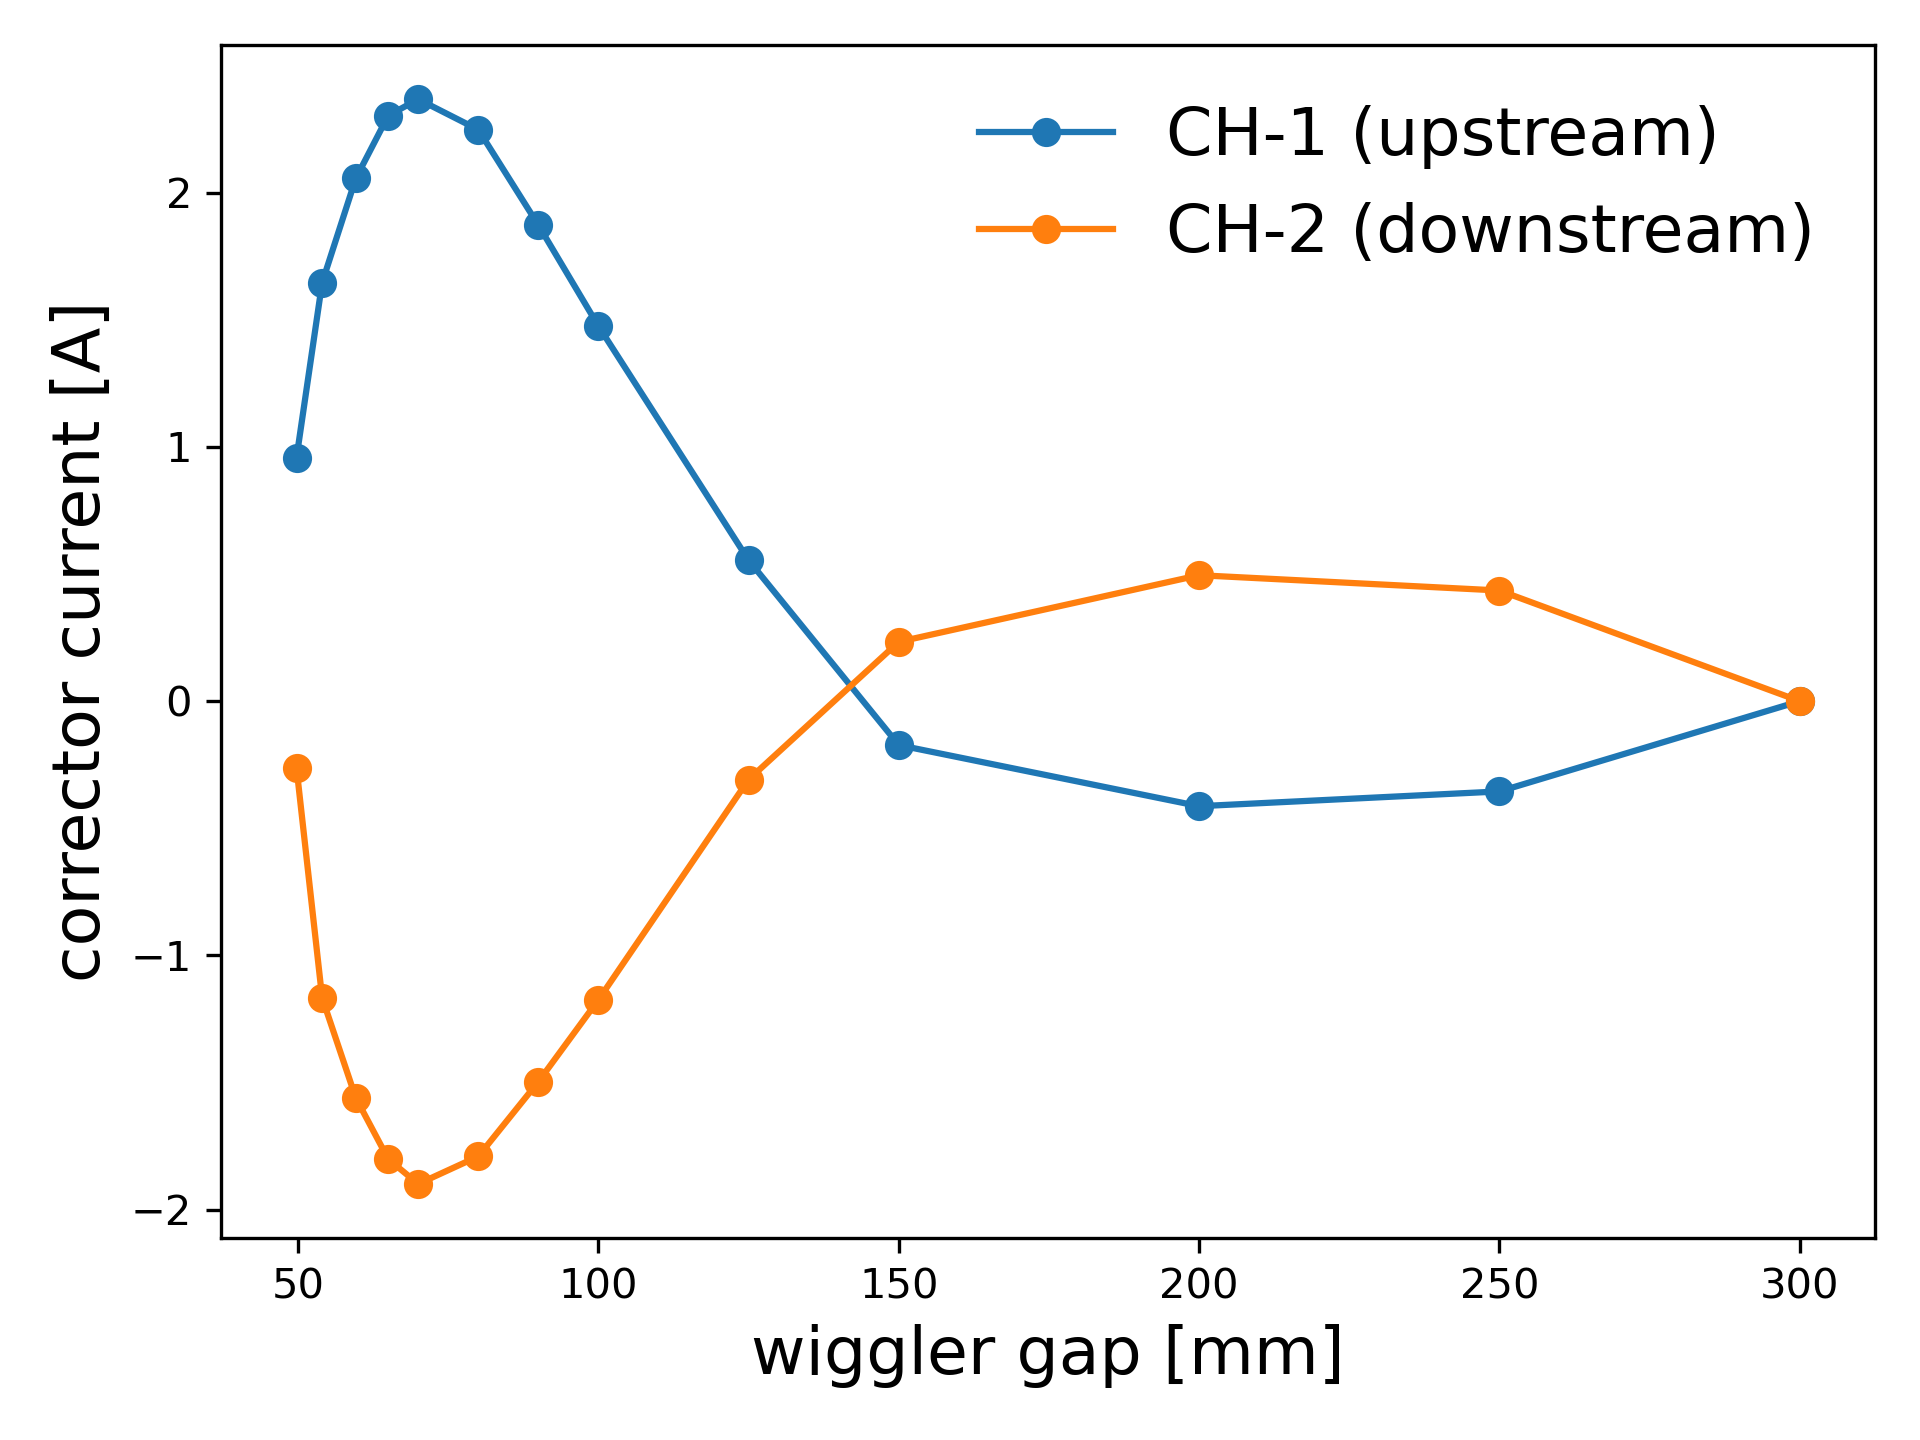
\includegraphics[width=0.49\textwidth]{wiggler_ffwd_table_new.png}
    \caption{Corrente das corretoras do wiggler necessárias para corrigir a distorção de órbita em função do gap. Os dados do gráfico estão na Tabela}
    \label{fig:ffwd_table}
\end{figure}

Para calcular o campo efetivo em função do gap podemos usar a equação que foi ajustada baseada em medidas:
\begin{equation}
    B_{\mathrm{eff}}\left(g\right) = 2.76 e^{-3.92 g\slash \lambda} + 0.01 \hspace{0.2cm} \mathrm{[T]}
\end{equation}
onde $g$ é o valor do gap em mm e $\lambda$ o período do wiggler também em mm. Para o wiggler W180 instalado, $\lambda = \SI{180}{\milli\meter}$.


\end{document}
